%!TEX root = main.tex
  \section{Related Work\label{sec:relatedworks}}
  % \subsection{Background and Motivation}
  \npar We will now describe past work in visual query systems and existing evaluation methods of visualization systems to provide background and motivation for our work. \cut{Then, we will introduce Pirolli and Card's sensemaking model, which serves as a framework for contextualizing our study findings.}
  % Visual query systems enable users to directly search for visualizations matching certain patterns through an intuitive specification interface. Early work in this space focused on interfaces to search for time series with specific patterns.
  % \change{For example, since} the intent of a sketch can be ambiguous, follow-up work has developed mechanisms to enable users to clarify how a sketch should be interpreted~\cite{ryall2005querylines,correll2016semantics,Mannino2018,Eichmann2015,Holz2009}.\dor{Should we move this sentence to the related work section?}
  \par \stitle{Visual Query Systems: Definition and Brief Survey}
  \npar The term \emph{visual query system} (VQS) was introduced by Ryall et al.~\cite{ryall2005querylines} and Correll and Gleicher~\cite{correll2016semantics} to describe systems that enable analysts to directly search for time-series\footnote{In this paper, we use this term to encompass line charts in general, since one of our domains (material science) does not visualize time on the x-axis.} visualizations matching a queried pattern, constructed through a visual specification interface. Examples of such systems include TimeSearcher~\cite{Hochheiser2001,Hochheiser2004}, where the query specification mechanism is a rectangular box, with the tool filtering out all of the time series that do not pass through it, and QuerySketch~\cite{wattenberg2001sketching} and Google Correlate~\cite{mohebbi2011google}, where the query is sketched as a pattern on canvas, with the tool filtering out all of the time series that have a different shape. Subsequent work, including TimeSketch~\cite{Eichmann2015}, SketchQuery~\cite{correll2016semantics}, and Qetch~\cite{Mannino2018}, recognized the ambiguity in sketching by studying how humans rank similarity in patterns. Finer-grained specification interfaces and pattern-matching algorithms have also been developed to improve the expressiveness of sketched queries and clarify how a sketch should be interpreted. These VQSs include QueryLines~\cite{ryall2005querylines} where queries can be flexibly composed of soft constraints and preferences and SoftSelect~\cite{Holz2009} where users can vary the level of sketch similarity across a search pattern. Beyond sketching, \zv~\cite{Siddiqui2017,Siddiqui2017VLDB}, SketchQuery, and TimeSearcher allow users to submit an existing visualization as the query, either via drag-and-drop or double-clicking on the existing visualization. In our work, we built on our existing system, \zv, since it was open-source, extensible, and included features beyond pattern and match specification typically found in existing systems, as compared in Table~\ref{table:relatedwork}. %\dor{I didn't incorporate Aditya's comment on stating that ``(the details of each component is described in Section~\ref{sec:pd_findings})'' here because it is already stated in the Table caption.}
  %with the system returning visualizations that had the closest Euclidean distance to the queried pattern. 
  % and described in Section~\ref{sec:sensemaking}. 
  %performed crowdsourced perceptual studies to understand how humans rank similarity in patterns subjectively
  % , including the use of soft constraints~\cite{ryall2005querylines} and implicit relaxed selection techniques~\cite{Holz2009}.
  % In addition to this ongoing work, recent work have also performed crowdsourced perceptual studies to understand how humans rank similarity in patterns subjectively~\cite{Eichmann2015,correll2016semantics,Mannino2018}.
  \begin{table}[ht!]
    \vspace*{-10pt}
     \centering
     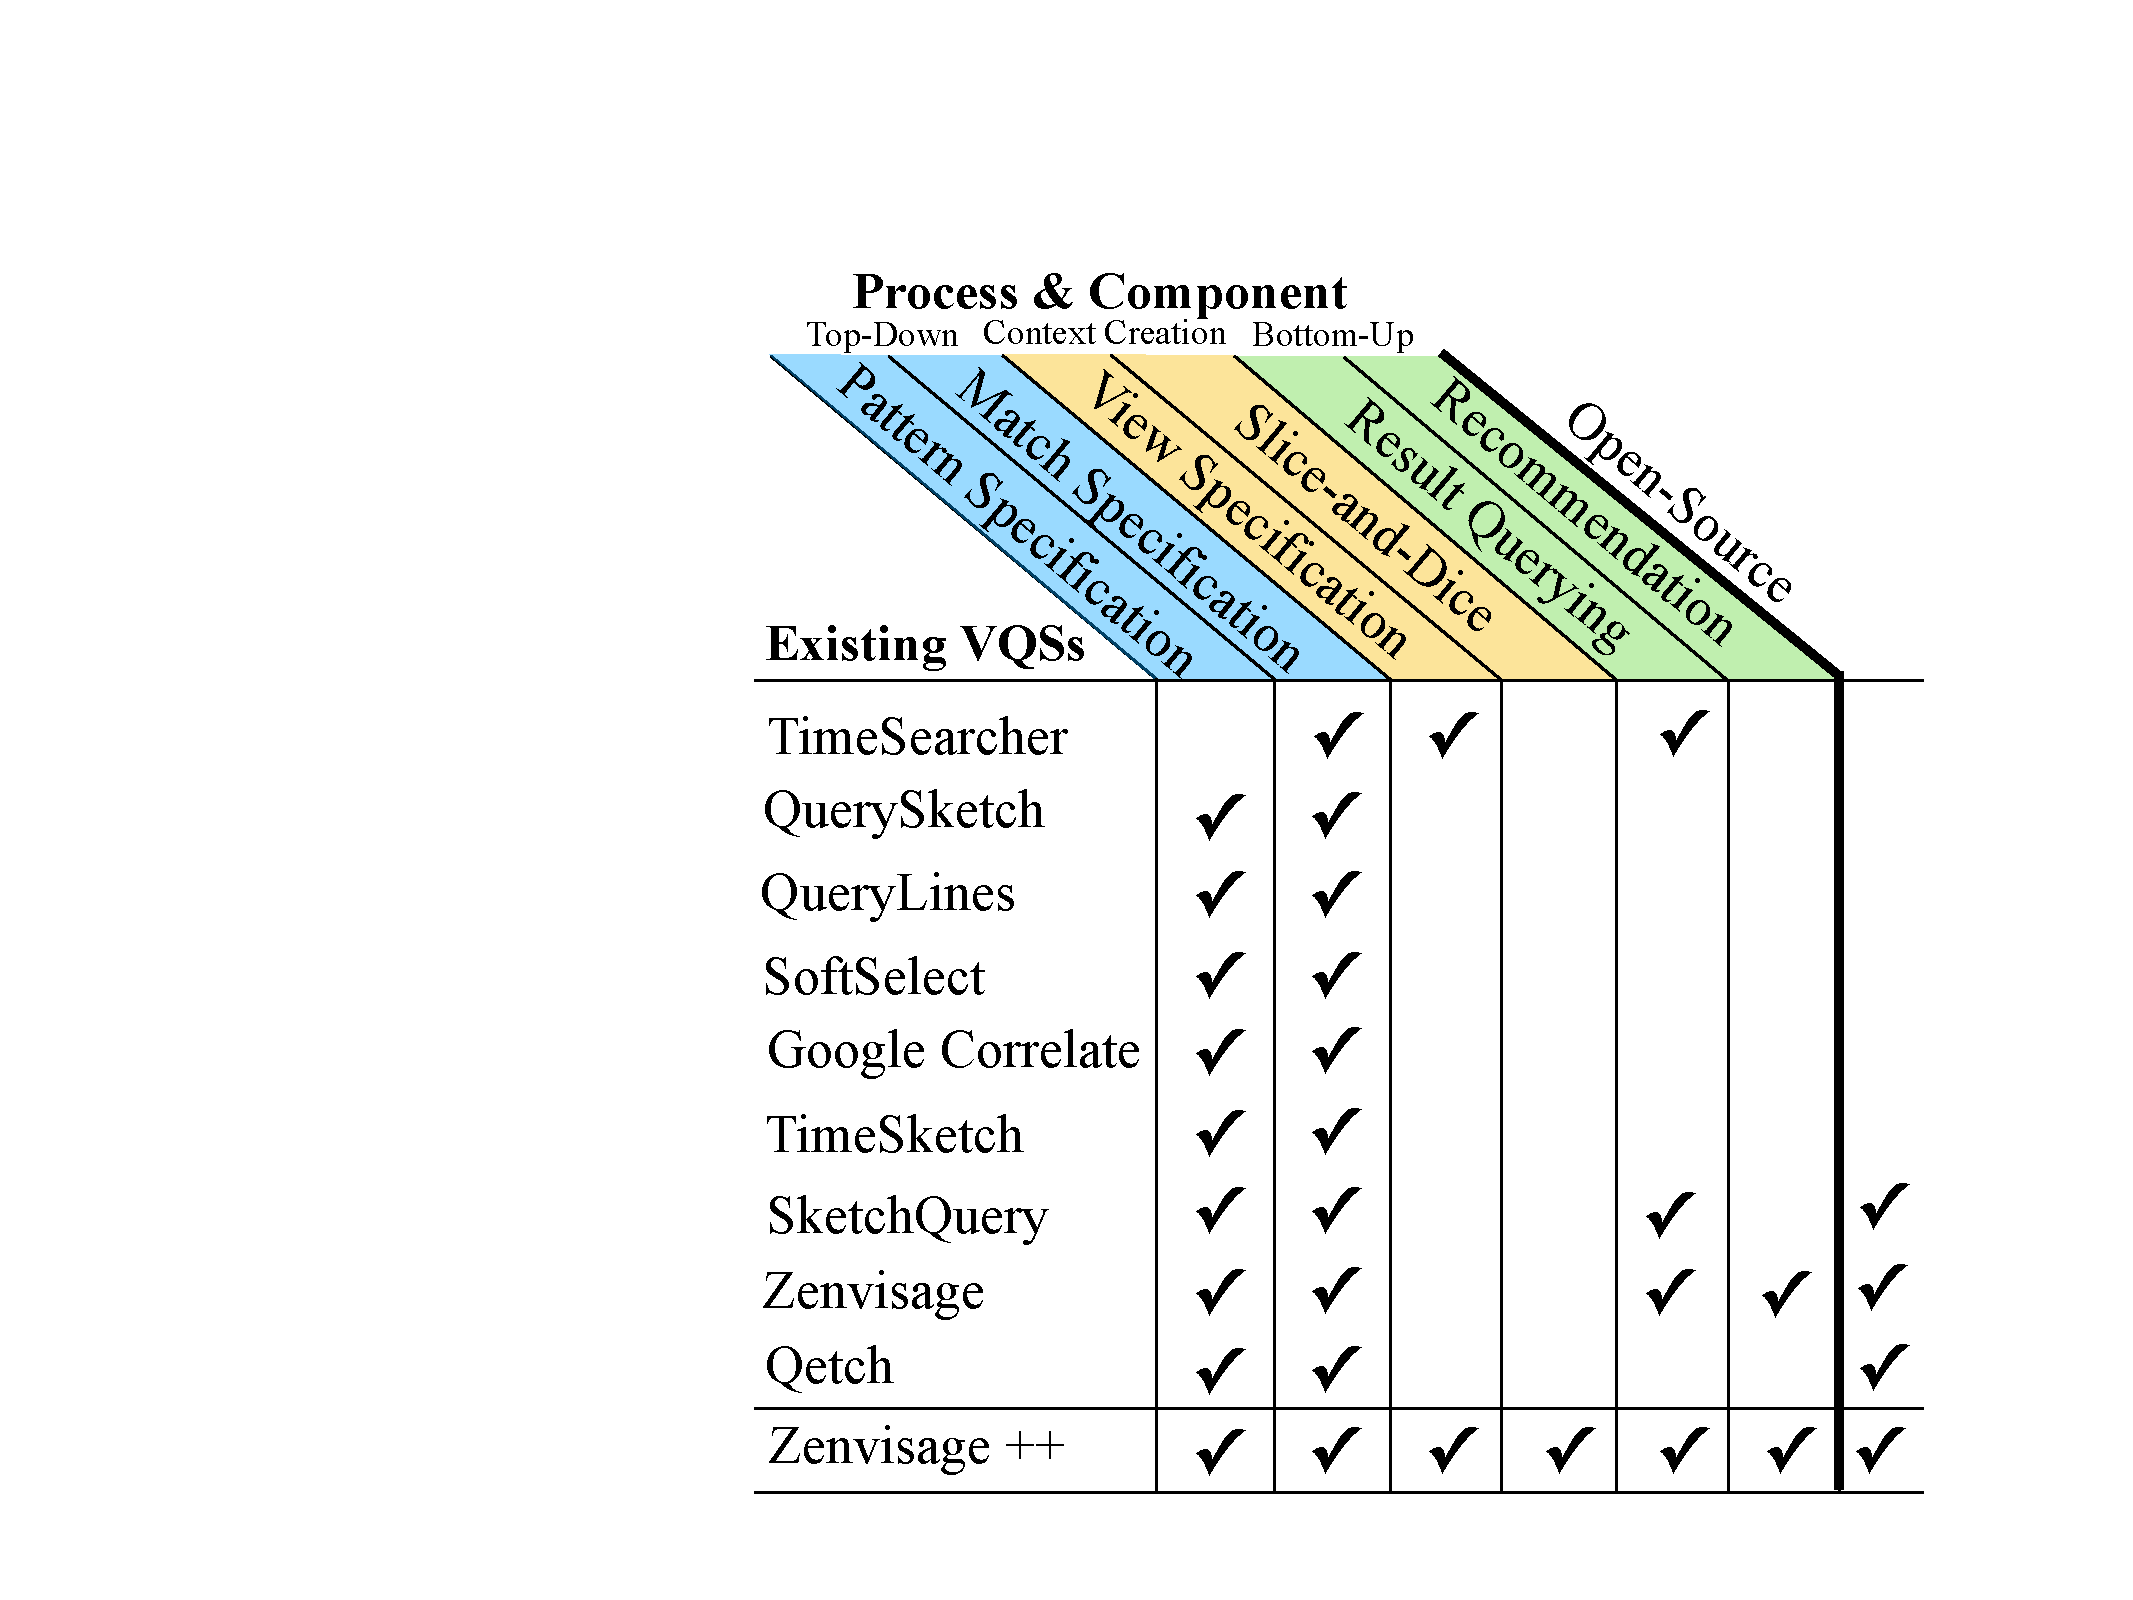
\includegraphics[width=0.8\linewidth]{figures/related_works_table.pdf}
     \caption{Table summarizing whether key functional components (columns) are covered by past systems (row, ordered by recency), indicated by checked cells. Column header colors blue, yellow, green represent three sensemaking process (top-down querying, search with context, and bottom-up querying) described in Section~\ref{sec:pd_findings}. The heavily-used, practical features in our study for context-creation and bottom-up inquiry is largely missing from prior VQSs.}
     \label{table:relatedwork}
     \vspace*{-10pt}
  \end{table}
  \par \stitle{Design and Evaluation Methodologies for Visualization Systems}
  \npar Visualization systems are typically evaluated via in-lab usability studies or controlled studies against existing visualization baselines~\cite{Plaisant2004,North2006,Yi2008}. However, successful lab-tested systems do not always translate to community acceptance and adoption. For instance, while decades of work have shown VQSs to be effective in controlled lab studies, they have not gained widespread adoption.\ccut{Unlike our work, past VQSs have never been designed and evaluated in-situ on multiple real-world use cases. Even when use cases were involved~\cite{Hochheiser2004,correll2016semantics}, the inclusion of these case studies served as a post-hoc demonstrative case study that had little influence on the major design decisions of the system.} The unrealistic nature of controlled studies has prompted the visualization research community to develop more participant-centered, ethnographic approaches for understanding how analysts perform visual data analysis and reasoning~\cite{Plaisant2004,lam2012empirical,shneiderman2006strategies,munzner2009nested,Sedlmair2012}. For example, multi-dimensional, in-depth, long-term case studies (MILCs) combine interviews, surveys, logging, and other empirical artifacts to create a holistic understanding of how a visualization system can be used in its intended environment \cite{shneiderman2006strategies}. 
  \par In the VQS literature, even though the development and evaluation of advanced VQS algorithms and interactions has been well underway for many years, prior work has yet to characterize and understand the needs of target users and observe how VQSs may be used as part of a real-world workflow, in order to address the initial questions of: 1) whether the problems that VQSs aim to address are even the right ones to address and 2) whether the chosen operations actually solve the user's problems. In the context of Munzner's nested model for visualization design and evaluation~\cite{munzner2009nested}, this gap between research and adoption stems from the common ``\textit{downstream threat}'' of jumping prematurely into the deep levels of \textit{encoding, interaction, or algorithm design}, before a proper \textit{domain problem characterization} and \textit{data/operation abstraction design} is performed. Our work fills this crucial gap in the existing literature and highlights how incorrect assumptions adopted by most prior work in this space regarding the first two stages of Munzner's model may have led to the present-day failures in VQS adoption.
  %to more deeply involve users in the co-design of an end-product (\zvpp) that they may eventually use.
  \par We performed design studies~\cite{lam2012empirical,shneiderman2006strategies,Sedlmair2012} with three different subject areas for \textit{domain problem characterization} by adopting \rchange{user-centered design practices with participatory design elements}. \rchange{User-centered design (UCD)~\cite{Norman1986,Nielsen1994,Gould1983} is a well-established method for iteratively designing a product that fits the need and desires of the user. In UCD, users assume a more passive role in conveying their needs to informing design decisions, but ultimately the design solutions are generated by the researcher/designer. We chose a mixed-methods approach that incorporated participatory design (PD) practices~\cite{Schuler1993,Muller1993} into UCD to engage potential stakeholders as co-designers early on and during every step of the design process, in order to develop a system that they may eventually adopt in their analytical workflows.} Participatory design is well-established in the CHI and CSCW community and has been successfully applied to develop systems for visual analytics~\cite{Aragon2008,Chuang2012}, tangible museum experiences~\cite{Ciolfi2016}, and scientific collaborations~\cite{Poon2008,Chen2016}. \cut{We chose to perform participatory design over other techniques for usability evaluation (such as long-term field study deployments or formative testing), since our goal was to engage potential stakeholders early on and in every step of the design process to ensure that design decisions are based on actual user needs and that we ultimately develop a system that may eventually be adopted in their analytical workflows.} 
  \par In order to ``\textit{[develop] a system model that will support [the] user's work}'' that subsequently ``\textit{fosters participatory design}'', Holzblatt and Jones~\cite{HoltzblattJones} describe contextual inquiry as a technique where researchers observe \rchange{participants} in their own work environment. Likewise, we first perform \rchange{contextual inquiry} and interviews with participants to understand their research questions and the challenges associated with their existing analytical workflows, and to identify design opportunities for VQSs. \cut{Past research has found that the use of functional prototypes is a common and effective way of engaging with participants, by providing a starting point for participatory design~\cite{Ciolfi2016}. Similarly, we provide a functional prototype at the beginning of the participatory design sessions to showcase the capabilities of VQSs.}\ccut{Since our participants were not aware of the existence of VQSs, let alone using them in their workflows, they would not have been able to imagine use cases for VQS without a starting point.} \cut{Likewise, the use of ``\textit{simulated future work situation}'' (where users are introduced to the envisioned use of the prototype) is prevalent in cooperative prototyping when the real use of the prototype is not feasible~\cite{Grnbak1991}.} To better understand how VQSs can be used in-situ participant's existing \rchange{workflows}, we regularly gathered feedback from participants and collaboratively envisioned potential designs based on preview demos of preliminary versions of our protoype \zvpp. \rchange{Based on our design findings, we contribute to the \textit{data/operation abstraction design} of VQSs in Munzner's model by developing a taxonomy for understanding how analysts make use of VQSs to accomplish their analytical tasks.} Finally, we validated our abstraction design with grounded evaluation~\cite{Plaisant2004,Isenberg2008}, where participants were invited to bring in their own datasets and research problems that they have a vested interest in to test our final deployed system.%\dor{Regarding Aditya's question on whether we could argue that PD is the only way to truly get at the heart ofthe problem underlying adoption. I don't think we should say this, there are many other possible techniques that Munzner's paper lists for dealing with domain and abstraction threats (for domain threats: ethnographic field studies, semi-structured interviews; for abstraction threats: formative testing collecting anecdotal evidence, long-term field study with deployed system). It would be hard to argue that PD is the *right* approach amongst these.}
  %Sedlmair et al. \cite{Sedlmair2012} highlights the benefits and pitfalls of design studies in visualization research. They advocate that design study methodology is suitable for use cases in which the data is available for prototyping, but the task is only partially known and the information is partially in the user's head. In that regard, our scientific use cases with VQS is well-suited for a design study methodology, as we learn about the scientist's data and analysis requirements and design interactions that helps users translate their ``in-the-head'' specifications into actionable visual queries. 
  %\par While these systems have been effective in controlled lab studies, they have never been designed and evaluated in-situ on multiple real-world use cases. Even when use cases were involved~\cite{Hochheiser2004,correll2016semantics}, the inclusion of these \change{case studies served as a post-hoc demonstrative case study that had} little influence on the major design decisions of the system. 
 %\change{Next, we will outline these two phases of our study, deferring details of the study procedures and protocols to the technical report.}%Next, we will describe these two phases of our study in more detail.
 \cut{
    \par \stitle{Sensemaking Models for Visual Analytics}
    \npar Based on our participatory design findings, we contribute to the \textit{data/operation abstraction design} of VQSs in Munzner's model by developing a taxonomy for understanding how analysts make use of VQSs to accomplish their analytical tasks. To develop a sensemaking model for VQSs, we draw from Pirolli and Card's \rchange{influential} paper on information sensemaking based on cognitive task analysis of intelligence analysts~\cite{Pirolli}. The sensemaking framework was designed to capture how expert analysts iteratively search and represent gathered evidence into a conceptual model (\emph{schema}). Many papers have applied this sensemaking framework to motivate tool designs, such as for exploratory browsing of visualizations in large datasets~\cite{Battle2016} and of the Web~\cite{Olston2003}. The sensemaking framework has also been used for understanding and modeling user behavior in visual analytics, such as how analysts gain insights from visualizations~\cite{Yi2008}, how biases can be introduced during visual analysis~\cite{Wall2017}, and how analysts transition between natural-language data facts and visualizations~\cite{Srinivasan2019}.
    \par In this framework, the sensemaking process can be organized into: 1) a foraging loop that searches for information to further schema organization and 2) a sensemaking loop for constructing a schema that best aligns with the insights obtained from the analysis. Overall, the model distinguishes between information processing tasks that are \textit{top-down} (from theory to data) and \textit{bottom-up} (from data to theory), described more in Section~\ref{sec:sensemaking}. We were inspired by this model for expert intelligence analysis as it bears semblance to our work for studying how domain experts perform exploratory visual analysis using VQSs.
  }
% Our VQS sensemaking model is inspired by Pirolli and Card's information foraging framework~\cite{Pirolli}, which distinguishes between information processing tasks that are \textit{top-down} (from theory to data) and \textit{bottom-up} (from data to theory).
% We analyze our participatory deisng findings through the lens of